\section{Project outcome}
\subsection{Preprocessing}
The three datasets have the same format audio file with the same label categories. Thus, I combined them into one dataframe for simplicity.  \\

Human emotion can be represented in terms of valence (pleasantness) and intensity [27]. For this implementation scenario, "Fear", "Disgusted", "Angry" and "Sad" are merged into a category as "Unpleasant" emotions, while "Happy", and "Surprised" are merged into another category as "Pleasant" emotions.
Finally, we would have 3 classes: "Pleasant", "Unpleasant", "Neutral".

\begin{center}
    \begin{figure}[!htp]
        \centering
        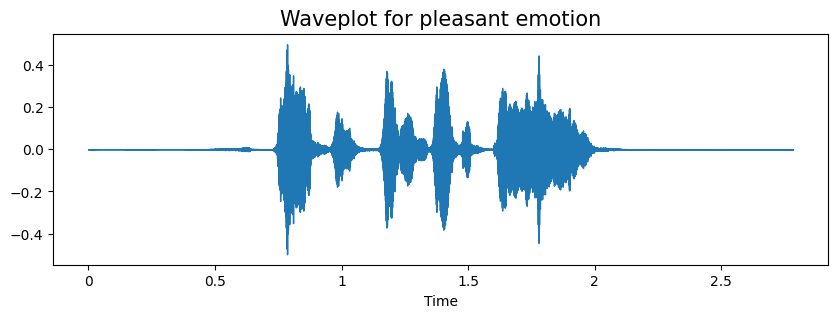
\includegraphics[width=0.8 \textwidth]{image/waveform_pleasant.png}
        \caption{waveform of pleasant emotion}
        \label{subsection}
    \end{figure}
    \end{center}

\begin{center}
    \begin{figure}[!htp]
        \centering
        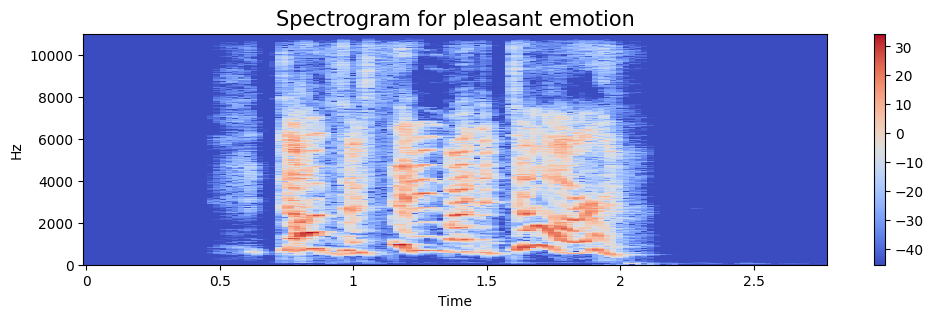
\includegraphics[width=0.8 \textwidth]{image/spectrogram_pleasant.png}
        \caption{spectrogram of pleasant emotion}
        \label{subsection}
    \end{figure}
    \end{center}

The detailed steps of preprocessing are as follows:

Emotion Label Encoding: The emotion labels are encoded to facilitate model training. This encoding step assigns numerical values to each unique emotion label.

\begin{itemize}
    \item Feature Extraction using MFCC: The audio data is transformed into Mel Frequency Cepstral Coefficients (MFCC) features. MFCC is a commonly used feature representation for speech and audio processing tasks. The outcome is a features matrix with shape (47, 13).
    \item Data Augmentation with Audio Transformations: The audio data is augmented by applying various audio transformations such as noise addition, time stretching, and pitch shifting. This augmentation technique increases the diversity of the training data and helps the model generalize better.
    \item Data Storage in CSV: The preprocessed data, including the encoded emotion labels and extracted MFCC features, is stored in a CSV file for easy access and further analysis.
    \item Data Split into Training, Validation, and Testing Sets: The preprocessed data is split into training, validation, and testing sets. This division allows for model training using the training set, hyperparameter tuning using the validation set, and final evaluation using the testing set.
\end{itemize}
    
\subsection{Model training & evaluation}

The model's structure is defined by adding layers sequentially. Two LSTM layers are incorporated, contributing to the model's ability to capture long-term dependencies. The first LSTM layer possesses 128 units and receives input with the specified input_shape. Additionally, it returns sequences to allow for subsequent processing. The second LSTM layer, with 64 units, further refines the representation of the input data.

To introduce non-linearity and increase model capacity, a dense layer with 64 units and a rectified linear activation function (ReLU) is included. This layer enables the model to learn complex relationships and extract meaningful features from the input data. To mitigate overfitting, a dropout layer with a dropout rate of 0.3 is inserted, randomly disabling connections between neurons during training.

For multi-class classification, a dense layer with 3 units and a softmax activation function is appended as the output layer. The softmax activation ensures the production of class probabilities, facilitating the assignment of the input to the most suitable class.

Upon defining the model, the code proceeds to compile it. An Adam optimizer, a widely used optimization algorithm, is employed with a learning rate of 0.001. The loss function chosen is sparse categorical cross-entropy, which is appropriate for multi-class classification tasks. The model's performance is evaluated using the accuracy metric.

After training, the model was evaluated with an accuracy of 76.15\% on the test set.
The confusion matrix shows that the model performs pretty fair for the 3 classes "Pleasant", "Unpleasant" and "Neutral", achieving precision of 77\%, 77\% and 71\%, respectively. 

This can be explained by the fact that the classes are merged from 6 classes to 3 classes, which makes the model easier to learn and predict. However, the accuracy is not high since I rescale the data samples, so the dataset is not large enough to train a good model.
    
\begin{center}
    \begin{figure}[!htp]
        \centering
        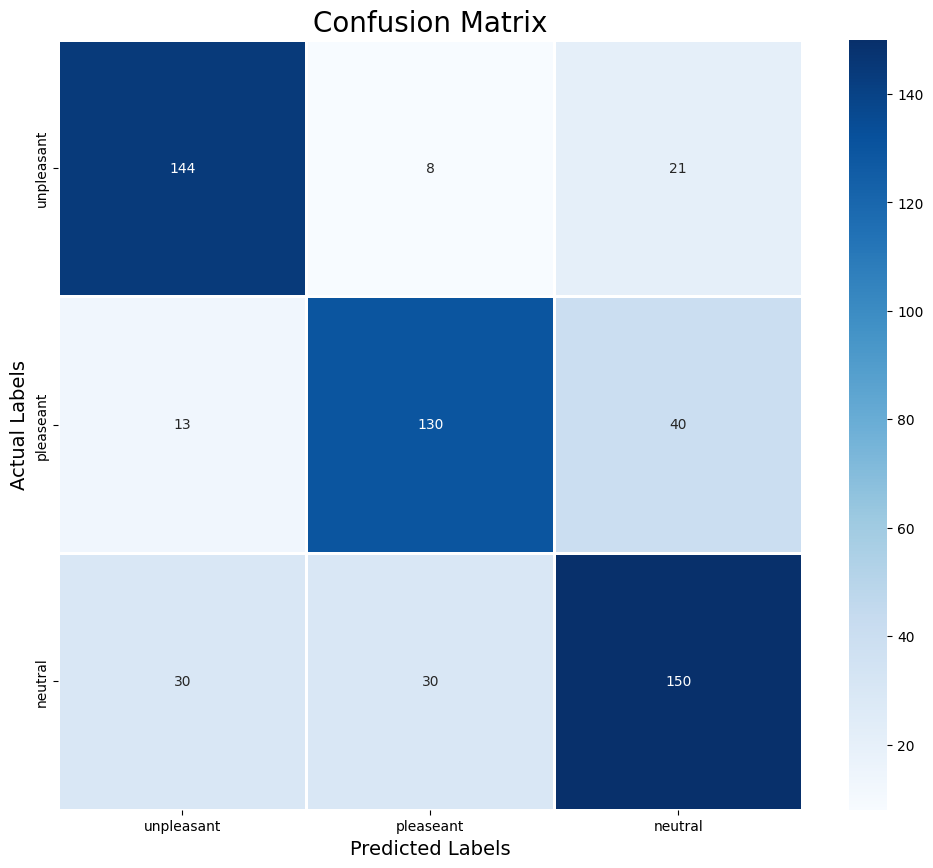
\includegraphics[width=0.8 \textwidth]{image/confusion_matrix.png}
        \caption{Confusion matrix}
        \label{subsection}
    \end{figure}
    \end{center}

\begin{center}
    \begin{figure}[!htp]
        \centering
        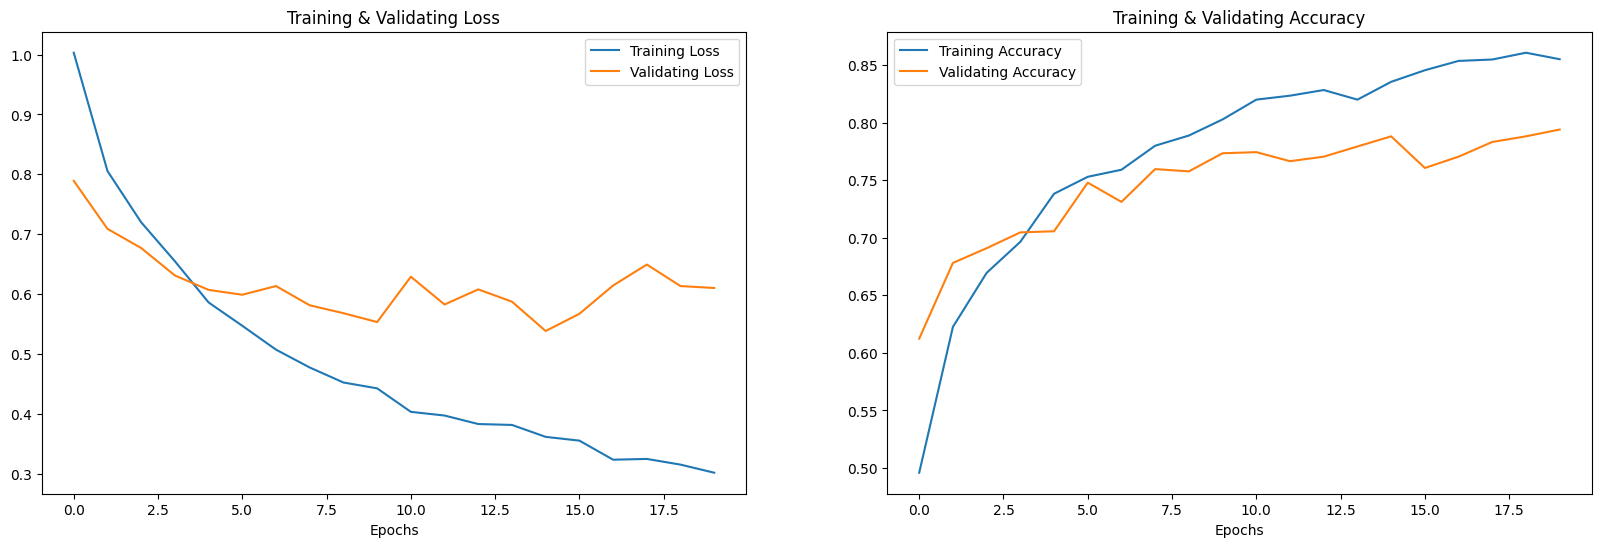
\includegraphics[width=0.8 \textwidth]{image/training_validating.png}
        \caption{Training \& validationresult}
        \label{subsection}
    \end{figure}
    \end{center}

\subsection{Model compression}
The objective of employing TinyML techniques is to minimize both the model size and inference time, while preserving a comparable level of accuracy.
Finally, I conduct a comparison between the inference time and accuracy of the original TensorFlow model and the TensorFlow Lite model. In this section, our objects are as follow:

\begin{itemize}
    \item Convert the model to tf lite model.
    \item Compare the size and the accuracy of models (before and after compress)
    \item Save the model in the format that deployable into suitable MCU
\end{itemize}

    \begin{table}[H]
        \centering
        \begin{tabular}{|l|l|l|l|}
            \hline
            \textbf{Reduce phase} & Size (byte) & Accuracy & Inference Time  \\ \hline
             original_model & 1568912 & 74.911660\% & 16.890739s \\
             tflite_model & 150032 & 74.558304\% & 0.413304 \\ hline
        \end{tabular}
        \caption{Reduce phase to find all books pair of books and number of users bought it}
        \label{tab:my_label}
    \end{table}

\\
\\
In conclusion, the TensorFlow Lite (TFLite) model demonstrates comparable accuracy to the original model while exhibiting notable improvements in model size and inference time. Despite its smaller size, the TFLite model maintains similar accuracy levels, making it an efficient and practical choice for deployment on resource-constrained devices. Additionally, the reduced inference time of the TFLite model allows for faster predictions, enhancing real-time performance in various applications. 
These benefits make TFLite an appealing solution for scenarios where optimizing model size and inference speed are critical considerations.